\subsection{Photons}
\label{sec:photons}

The kinematic requirements applied on the photons, after the diphoton candidates have passed through the event pre-selection (see Section ~\ref{sec:trigger}), are similar to the ones used in the SM $\Hgg$ analysis. The selection is as follows:
\begin{itemize}
\item Leading photon $E_{T} > 30 \GeV$, trailing photon $E_{T}>20 \GeV$;
\item Leading photon $E_{T}/\Mgg > 1/3$, trailing photon $E_{T}/\Mgg > 1/4$;
\item $100 < \Mgg < 180 \GeV$.
\end{itemize}
Additionally, a photon identification requirement is applied to the photons.

The photon identification requirement is based on a multivariate algorithm that combines information from the photon cluster shape in ECAL, as well as isolation variables. 
This requirement provides a signal-like photon efficiency of $90\%$ for photons both on the ECAL barrel and endcaps. 
The scale factors used to ensure data/MC agreement in the selection efficiency are also applied; these scale factors are calculated centrally at CMS. 
Additionally, an electron veto is applied to avoid background with electrons faking photons, with corresponding scale factors and uncertainties.

%=========== OLD ===========

%Currently (as of January 2016), the available samples processed by the $\Hgg$ group only have stored 
%their own training of the photon MVA ID. 
%We have chosen working points that ensure that the resonant low mass samples have 
%a $90\%$ efficiency both in the barrel and the endcap ECAL regions. 

%\begin{table}[h]
%\centering
%\begin{tabular} { | c | c | }
%\hline
%ECAL Region & Hgg MVA Selection \\ \hline
%EB & 0.07 \\ \hline
%EE & -0.03 \\ \hline
%\end{tabular}
%\end{table}

%Efficiencies of the leading photon to pass the ID criteria, as a function of the photon transverse energy, 
%are shown in Figure \ref{fig:Hgg-PhoID-eff}. 
%Only photons matched to gen-level prompt photons are used. 


%\begin{figure*}[thb]
%  \centering
%  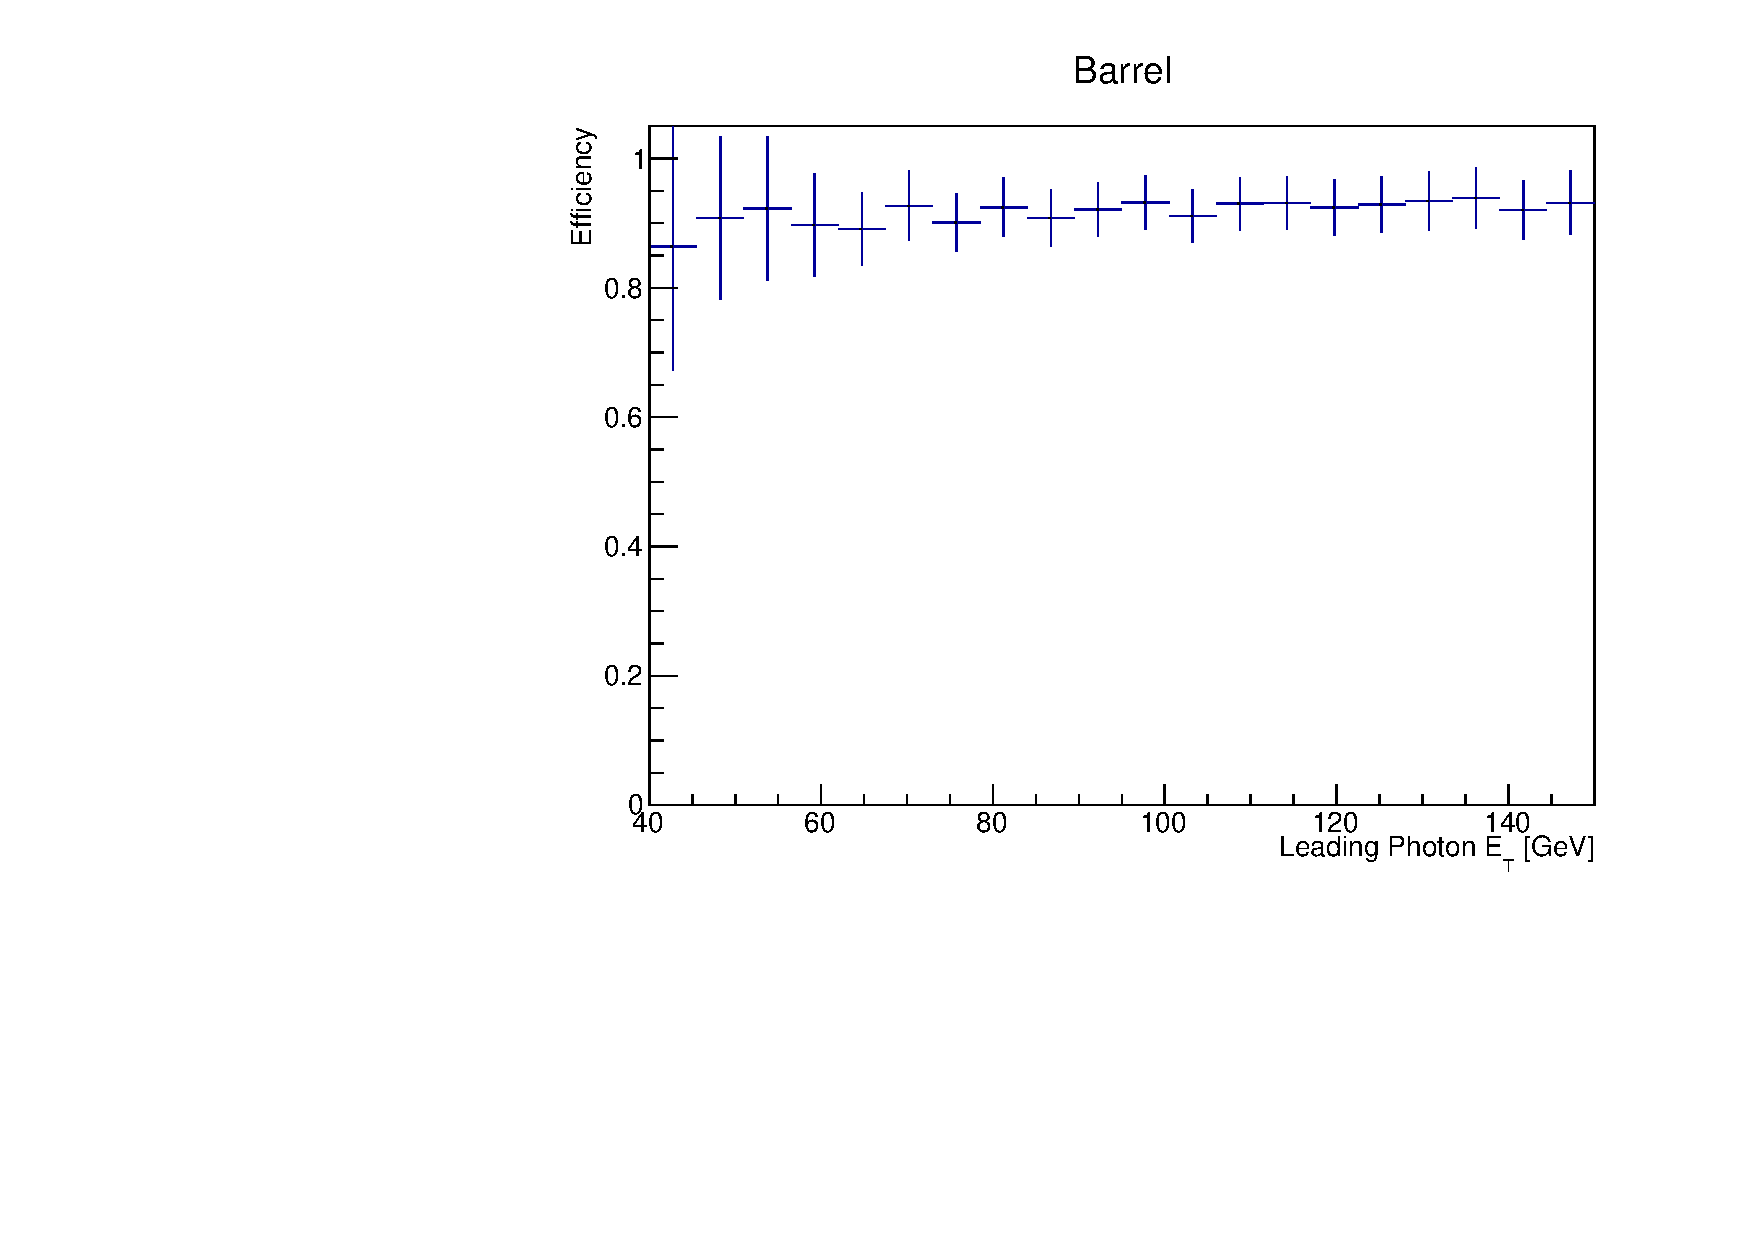
\includegraphics[width=0.45\textwidth]{figures/sec-photons/SMHH_HggMVA_Eff_EB.pdf}\hfil
%  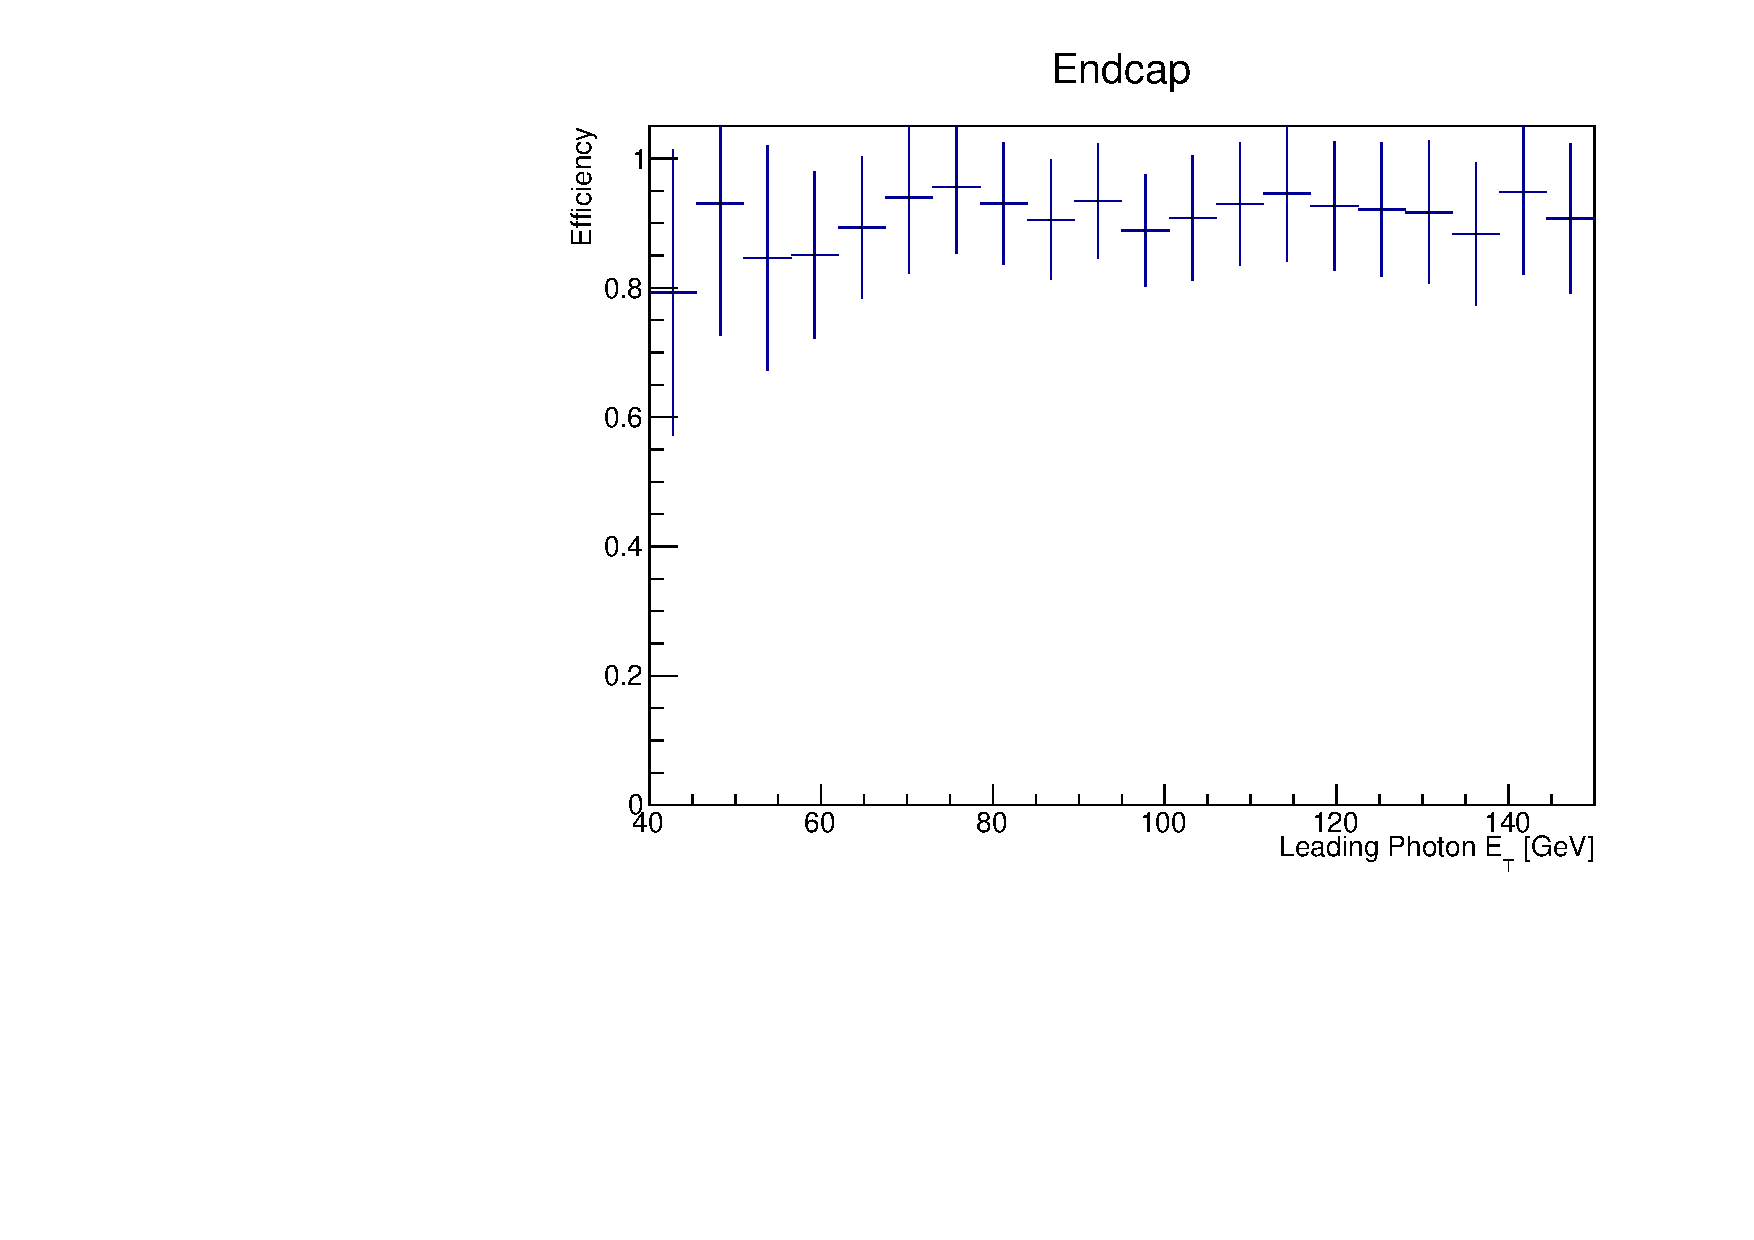
\includegraphics[width=0.45\textwidth]{figures/sec-photons/SMHH_HggMVA_Eff_EE.pdf}\hfil
%  \caption{Efficiencies of the leading photon to pass the ID criteria, as a function of the photon transverse energy, 
%for photons in the barrel and endcap regions of ECAL. }
%  \label{fig:Hgg-PhoID-eff}
%\end{figure*}

%We have studied all of those possibilities with MC samples, and for the 2015 data we
%decided to use the MVA ID of EGamma group with \textit{Loose} working point (WP),
%corresponding to 90\% signal selection efficiency.  A brief summary of this study is
%described below.

%The true photons are selected from the $G \to \HH \to \bbgg$ signal MC samples (they are
%required to match the generated level photons within $\Delta R< 0.1$ cone). The fake
%photons are selected from the Double-EM enriched $\gamma$+jet samples (and they must not
%to match to any generated level photon).
%The studied photons must pass the standard photon selection (pre-selection plus kinematic selection).

%Finally, the MVA score is calculated for the selected photons (or an ID decision for the
%cut-based ID).  Figure \ref{fig:phoID-MVA} shows two examples of the MVA output from the
%signal and fake photons. And Figure~\ref{fig:phoID-ROC} shows the ROC curves for the three
%IDs considered, for photons in the Barrel and Endcap. On these curves at a given signal
%efficiency one would prefer to have highest background rejection. From this figure of
%merit the MVA IDs are undoubtedly better than the cut-based ID. While the two MVA IDs have
%very similar performance.

%Note: it is anticipated that for 2016 data-taking the two MVA IDs will merge into one, and we
%will use that.

%\begin{figure*}[thb]
%  \centering
%  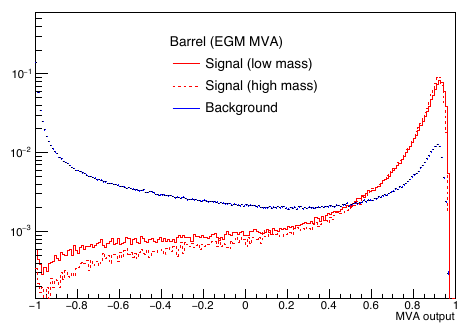
\includegraphics[width=0.45\textwidth]{MVA_output_EGM_Barrel}\hfil
%  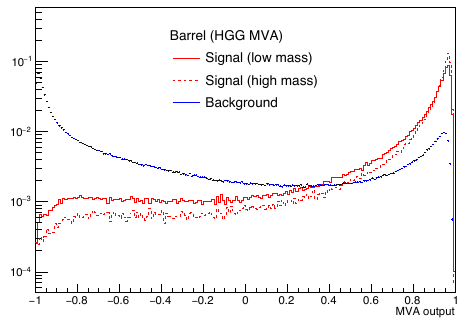
\includegraphics[width=0.45\textwidth]{MVA_output_HGG_Barrel}\hfil
%  \caption{Examples of the MVA ID outputs for the photons in the Barrel. Left: EGamma,
%    right: Hgg.}
%  \label{fig:phoID-MVA}
%\end{figure*}


%\begin{figure*}[thb]
%  \centering
%  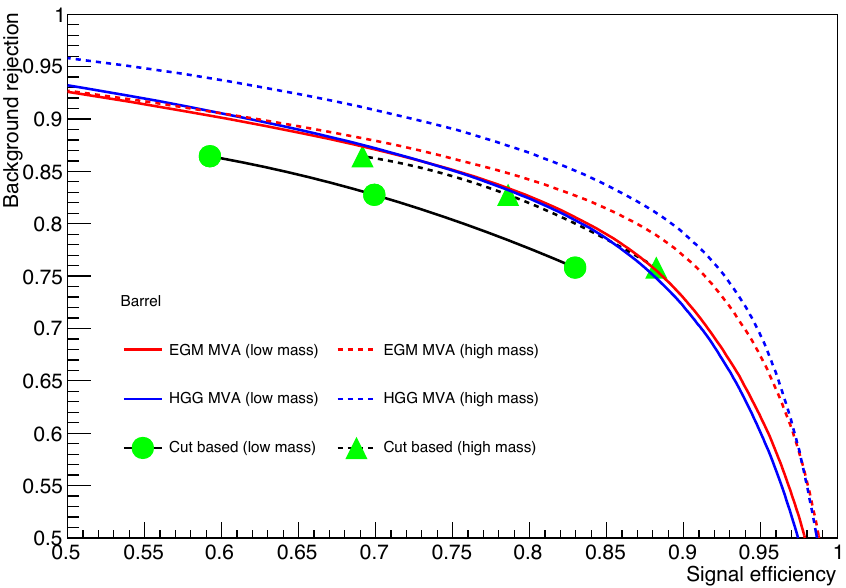
\includegraphics[width=0.45\textwidth]{ming_phoID_EB}\hfil
%  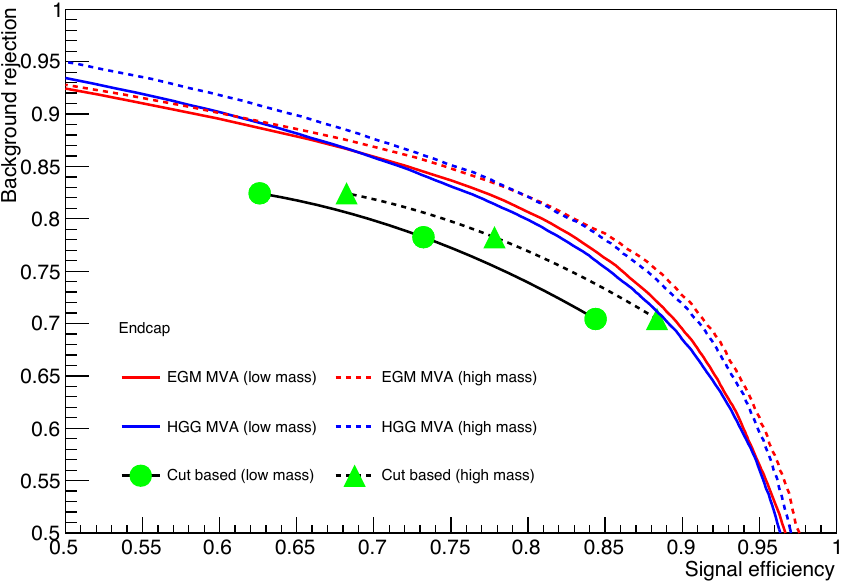
\includegraphics[width=0.45\textwidth]{ming_phoID_EE}\hfil
%  \caption{Photon ID ROC curves}
%  \label{fig:phoID-ROC}
%\end{figure*}

\subsubsection{Fake Photon Control Region}\label{sec:PCR}
A control region is created by selecting diphoton candidates with one photon that passed the ID requirement and one that didn't. All the other selections remain the same, and the procedure to select such diphoton candidates is the same as in the signal region. This control region is used in the analysis to perform closure tests on the background modeling.

\subsubsection{Vertex}
Inheriting from the main $\Hgg$ analysis, we use the vertex that gives the highest $\Hgg$ vertex MVA score. 
Because there are additional jets in the event,  picking this vertex has a very small mismatch efficiency. 
Only in less than $0.1\%$ of the events, the chosen vertex is different from the vertex associated to the true vertex in the simulation. 

The $\Hgg$ vertex MVA score is based on three variables calculated for each reconstructed vertex: the sum of the squared transverse momenta of the charged particle tracks associated with the vertex, and two variables that quantify the vector and scalar balance of $p_{T}$ between the diphoton system and the charged particle tracks associated with the vertex. 
In addition, if either photon is associated with any charged particle track that has been identified as resulting from conversion, the conversion information is also used. 
The variables are used as the inputs to a multivariate classifier based on a boosted decision tree (BDT) to choose the reconstructed vertex to be associated with the diphoton system. 
The average vertex finding efficiency of this algorithm in the SM $\Hgg$ analysis is $80\%$.

\subsubsection{Gain Switch}

In 2016, it was observed that high energy deposits in ECAL had their energies reconstructed with a certain bias, due to the shaping of the pulses in the ECAL VFE electronics. 
This shaping became a problem in Run 2 because we assume a certain shape for the signal amplitude from the crystals when measuring this amplitude, as described in the Multifit method. 
It has been observed that this bias occurs when an energy deposit is high enough to cause a gain switch in the ECAL multi-gain amplifier.

We investigated the fraction of selected events in our blinded signal region with photons that go through gain switches. 
The plots on Figure \ref{fig:gain_switch}  show, in bins of $\tilde{M}_{X}$, the fraction of events with at least one of the photon candidates going through gain switches (to gain 1, gain 6 or both). 
These results show that, for the high mass region, around $20\%$ of our events are affected by gain switches. 
This non-negligible rate means that the analysis needs to use the new CMS re-processed data in which the issue has been fixed.

\begin{figure*}[thb]
  \centering
%  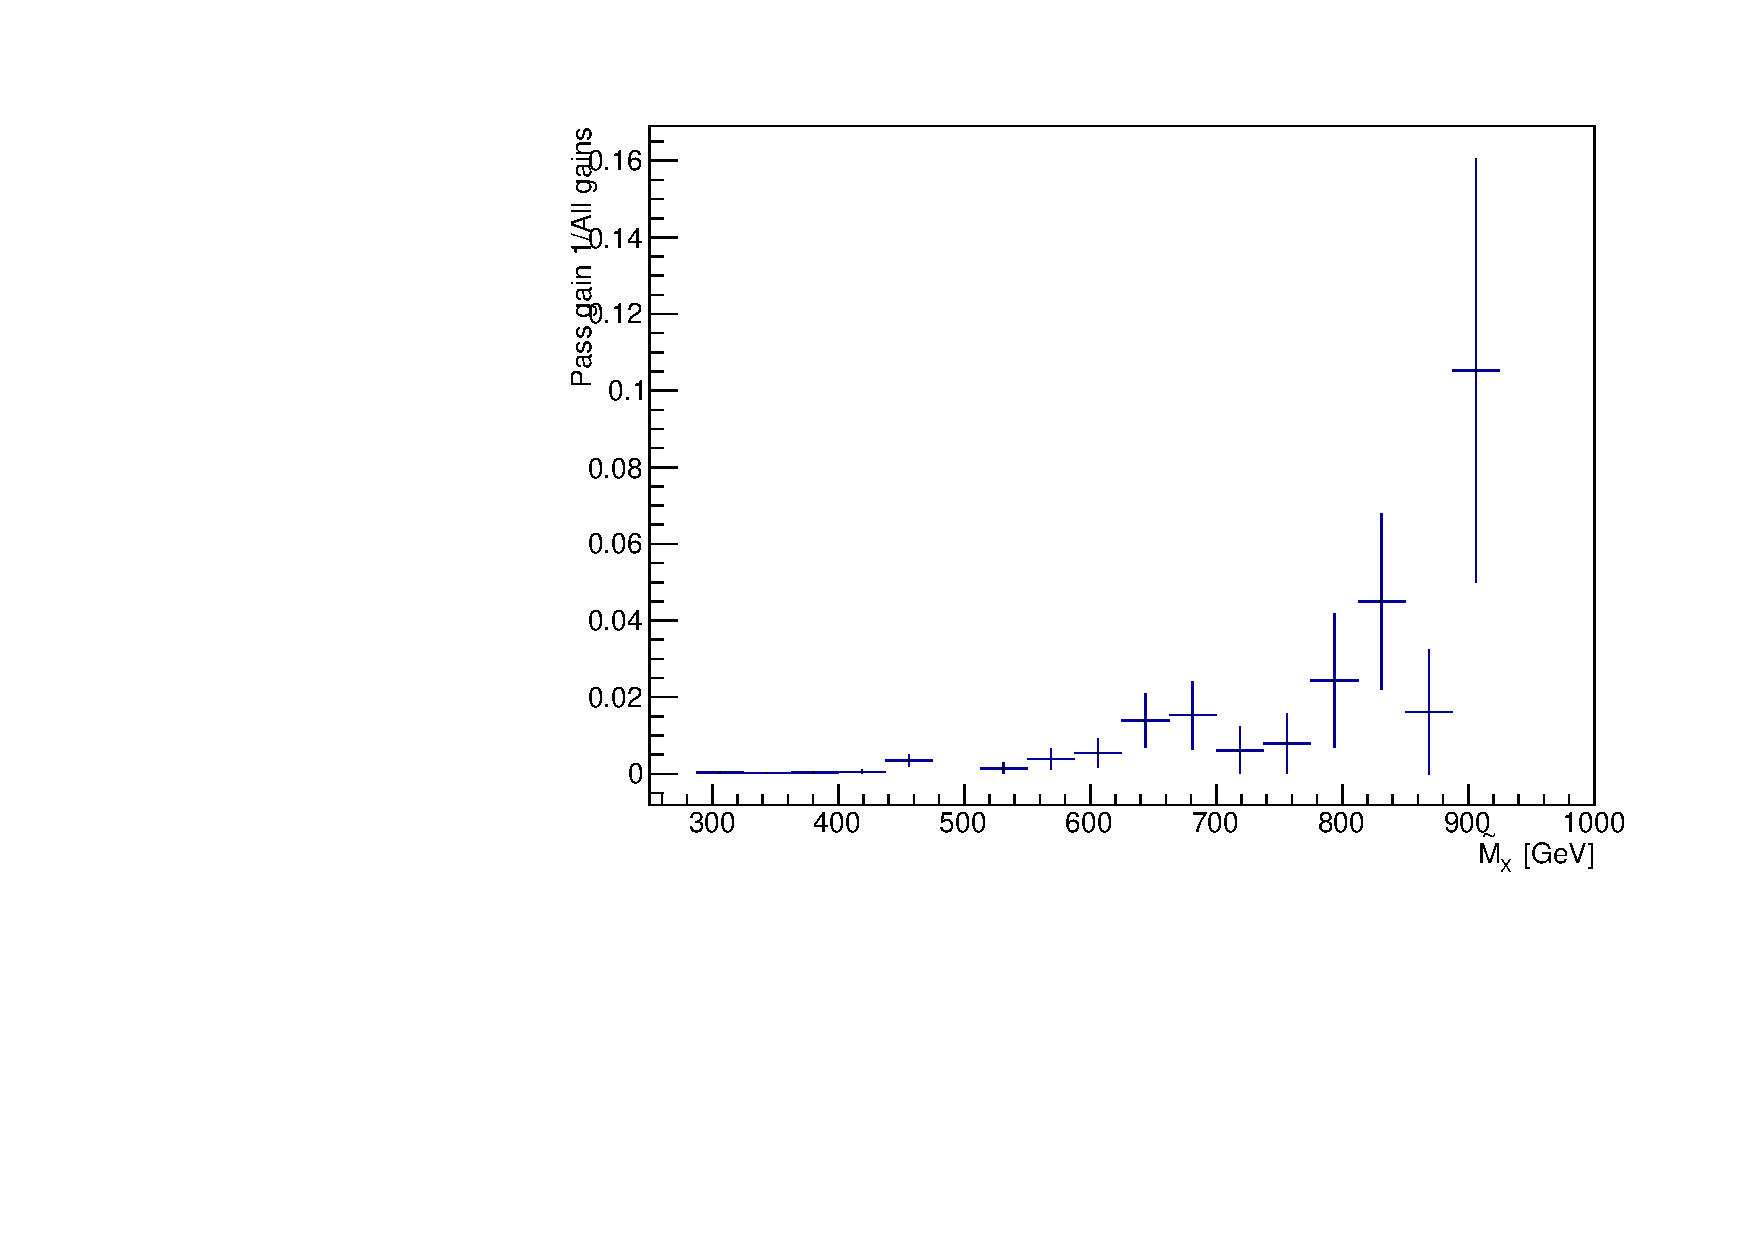
\includegraphics[width=0.3\textwidth]{figures/sec-photons/rg1}\hfil
%  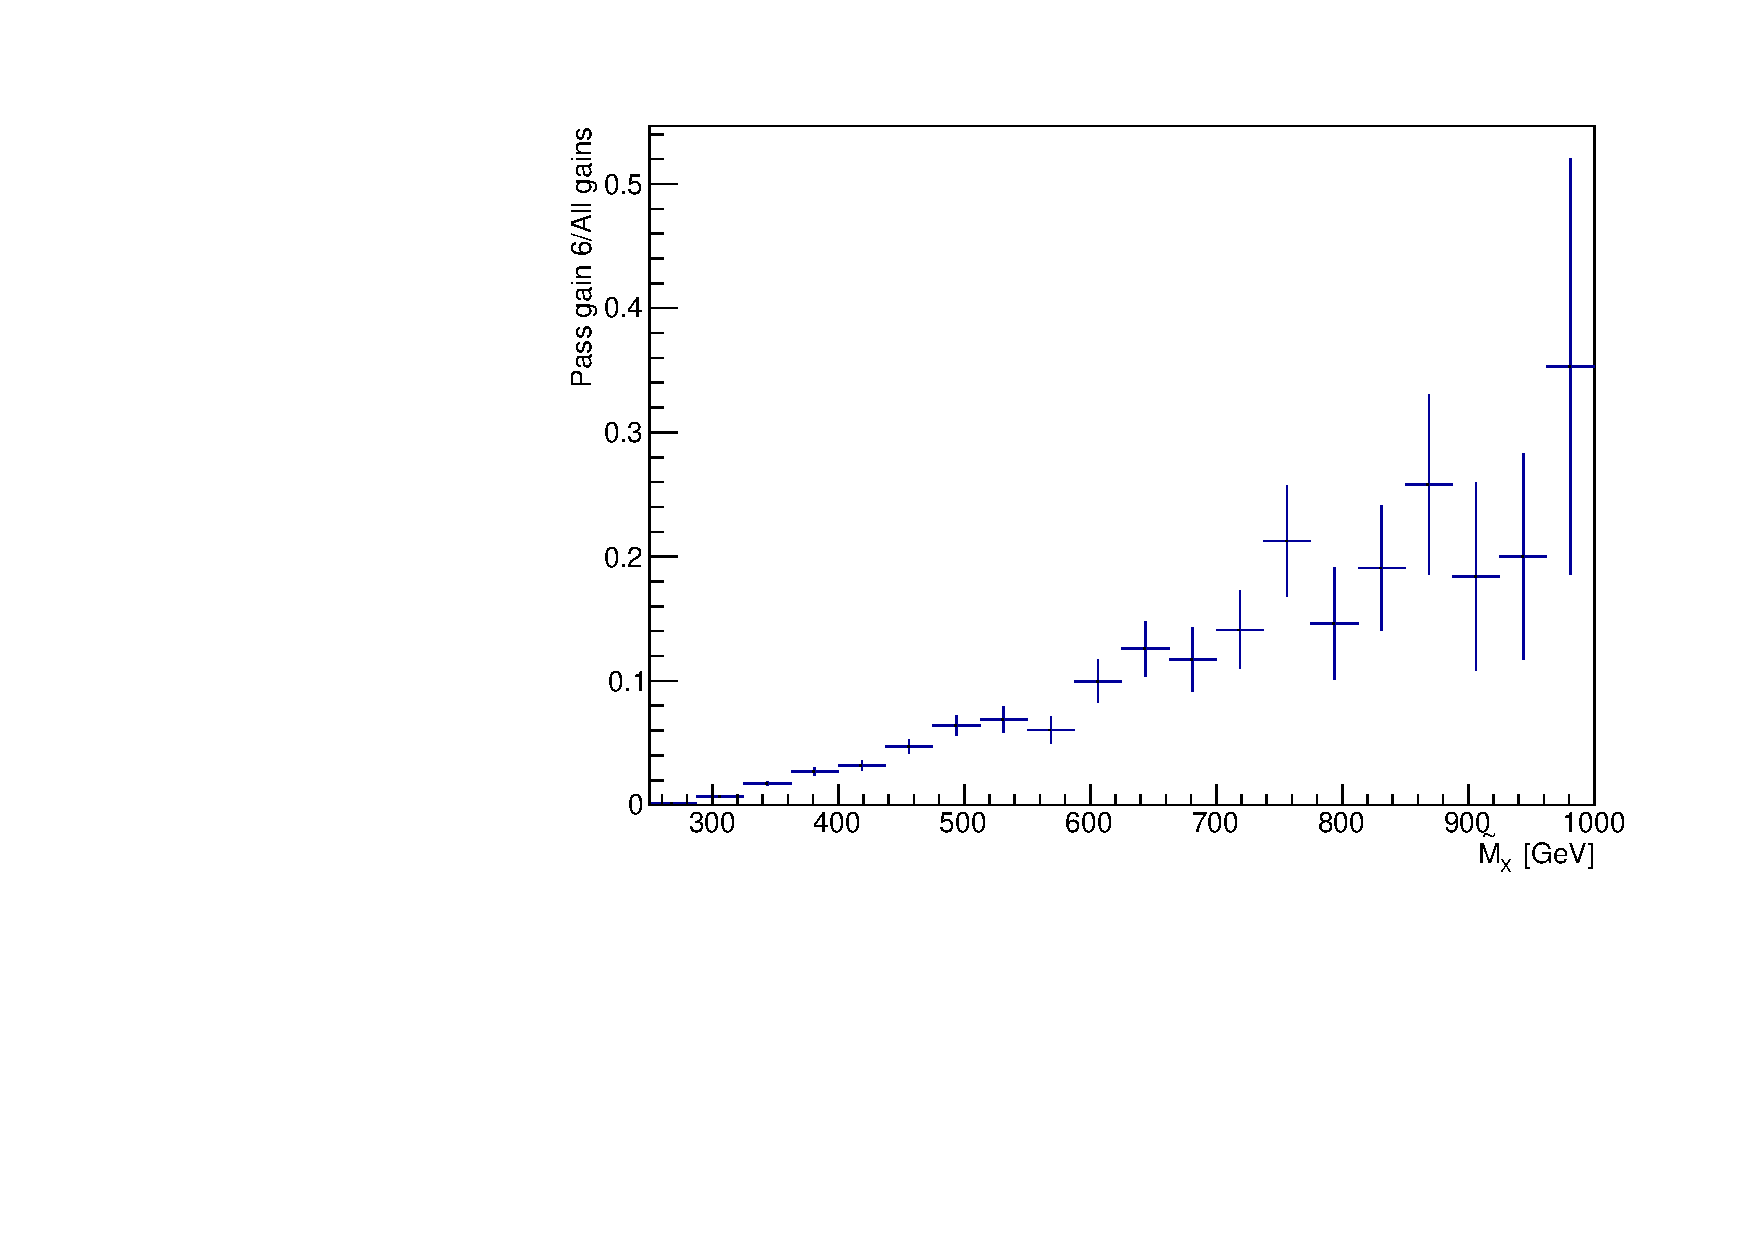
\includegraphics[width=0.3\textwidth]{figures/sec-photons/rg6}\hfil
  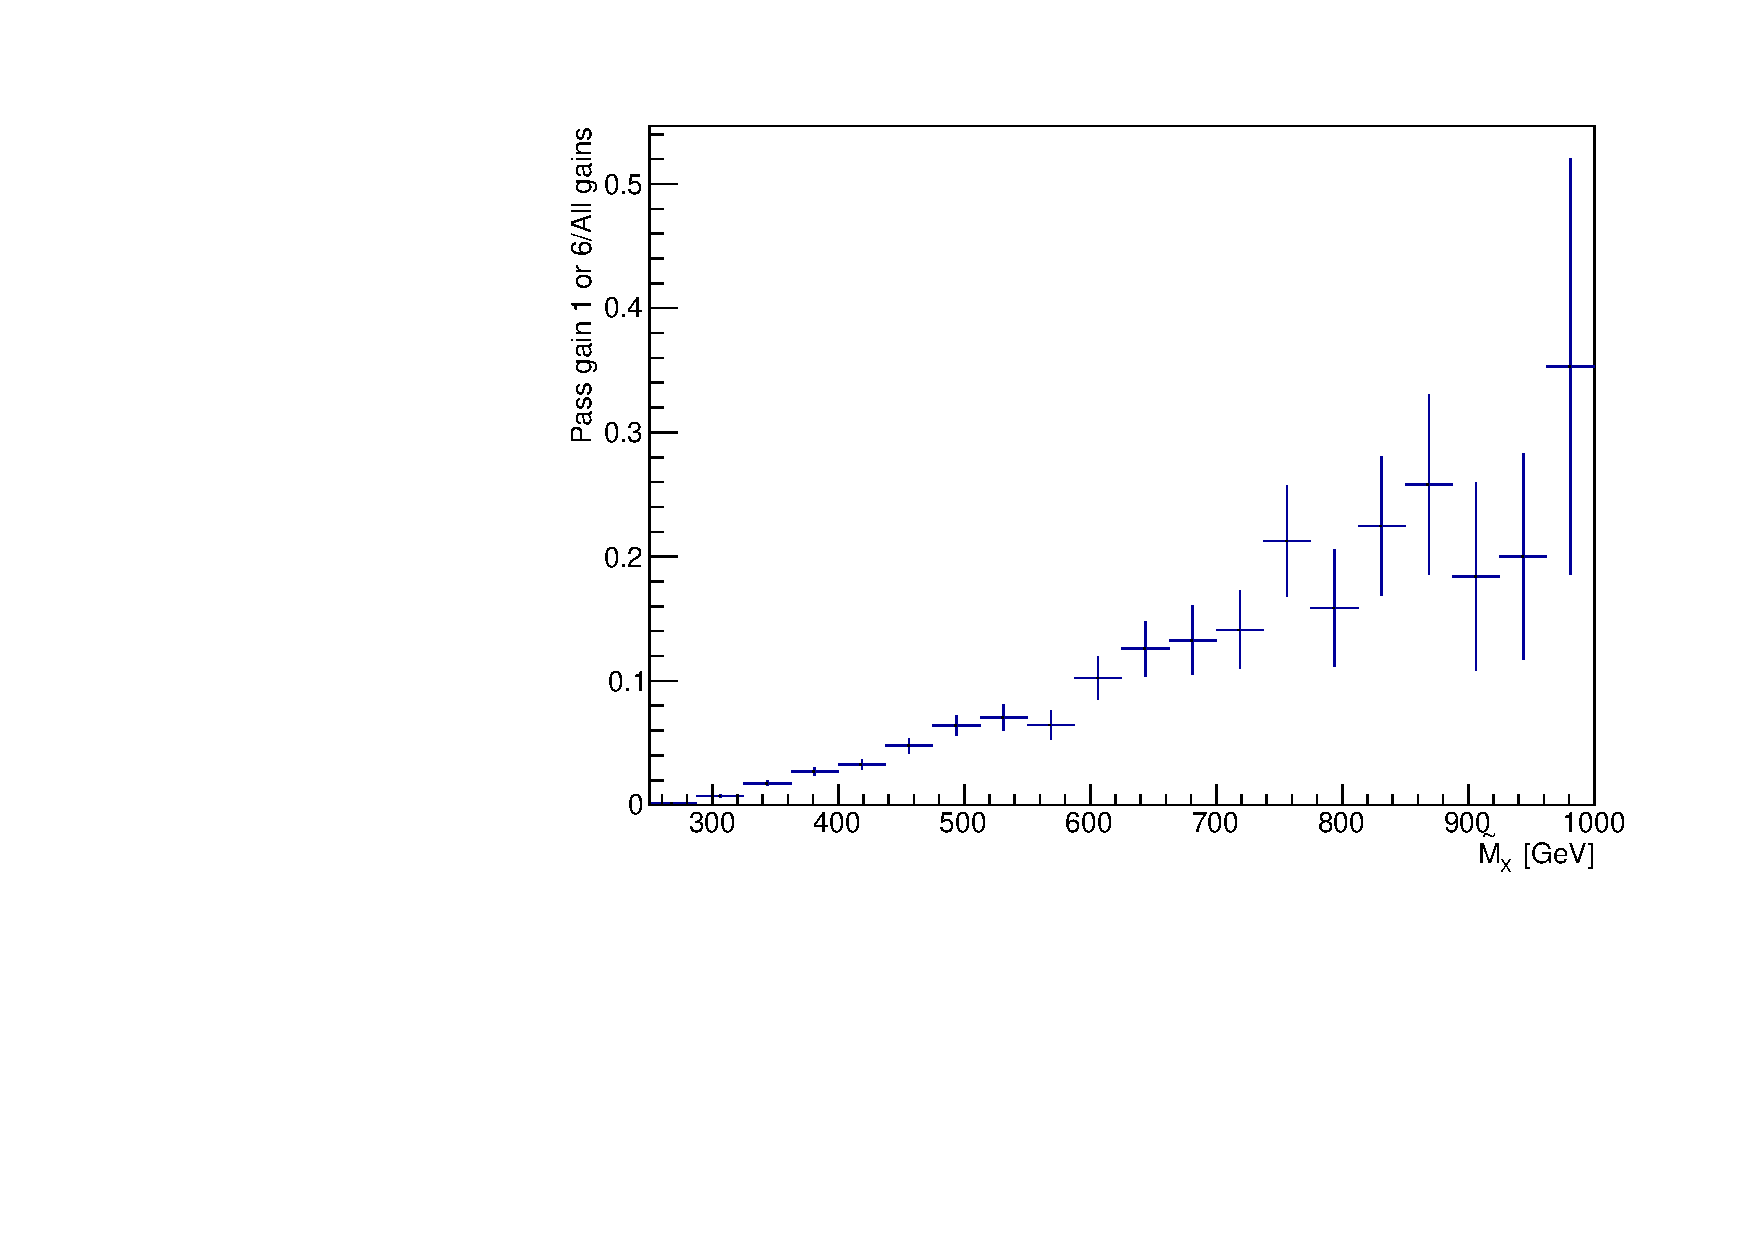
\includegraphics[width=0.5\textwidth]{figures/sec-photons/rg16}
  \caption{Fraction of events with photon candidates going through gain switch.}
  \label{fig:gain_switch}
\end{figure*}

\subsubsection{Regression}

A new version of the photon energy regression has been trained with the Run 2 data taking conditions. 
This regression aims to correct the photon super cluster energy, as described in previous sections.  
We compared this new regression to the previous training, as seen in the plots of Figure \ref{fig:pho_reg} for three different resonance mass points. 
The difference observed is not large enough for this analysis to be affected, so the previous regression version is used (following main $\Hgg$ analysis).

\begin{figure*}[thb]
  \centering
  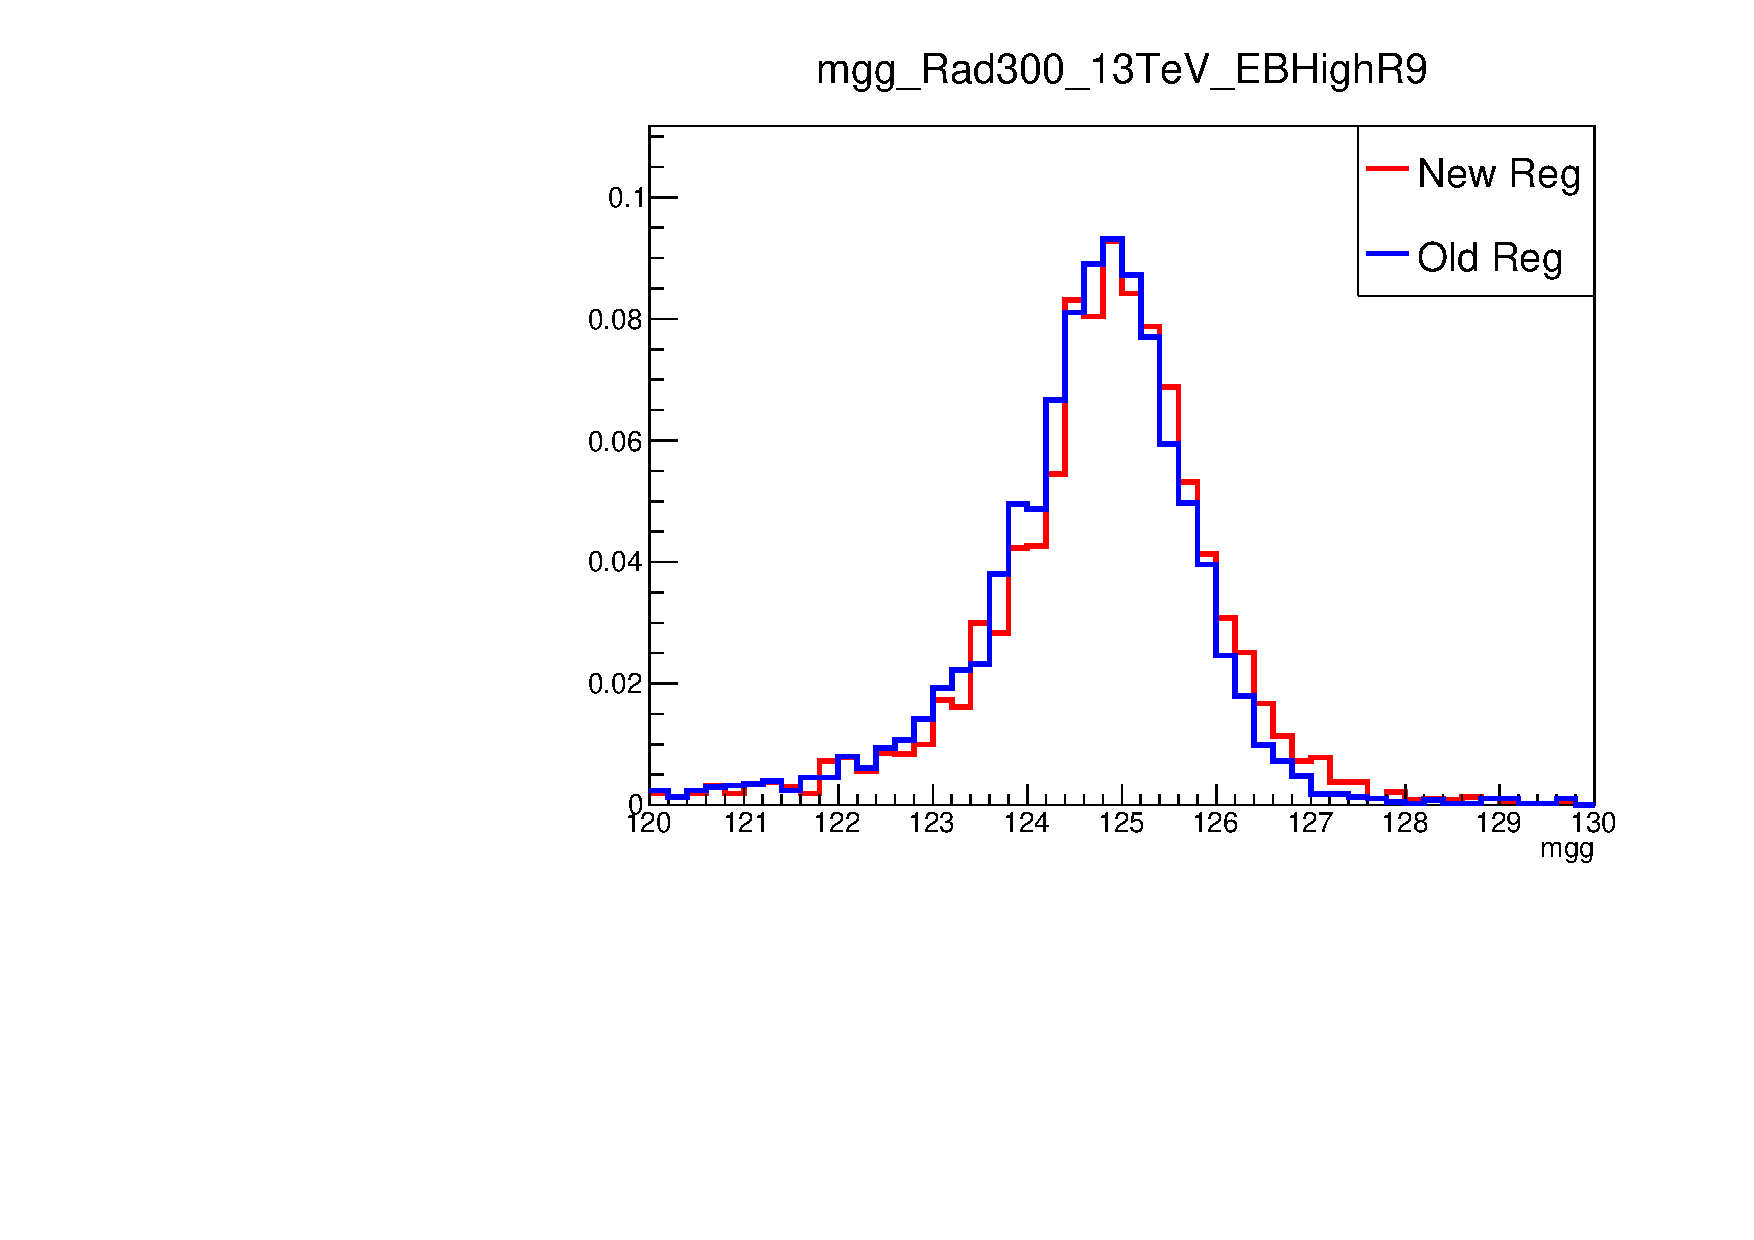
\includegraphics[trim={0 0 0 0.95cm},clip,width=0.3\textwidth]{figures/sec-photons/mgg_Rad300_13TeV_EBHighR9.pdf}\hfil
  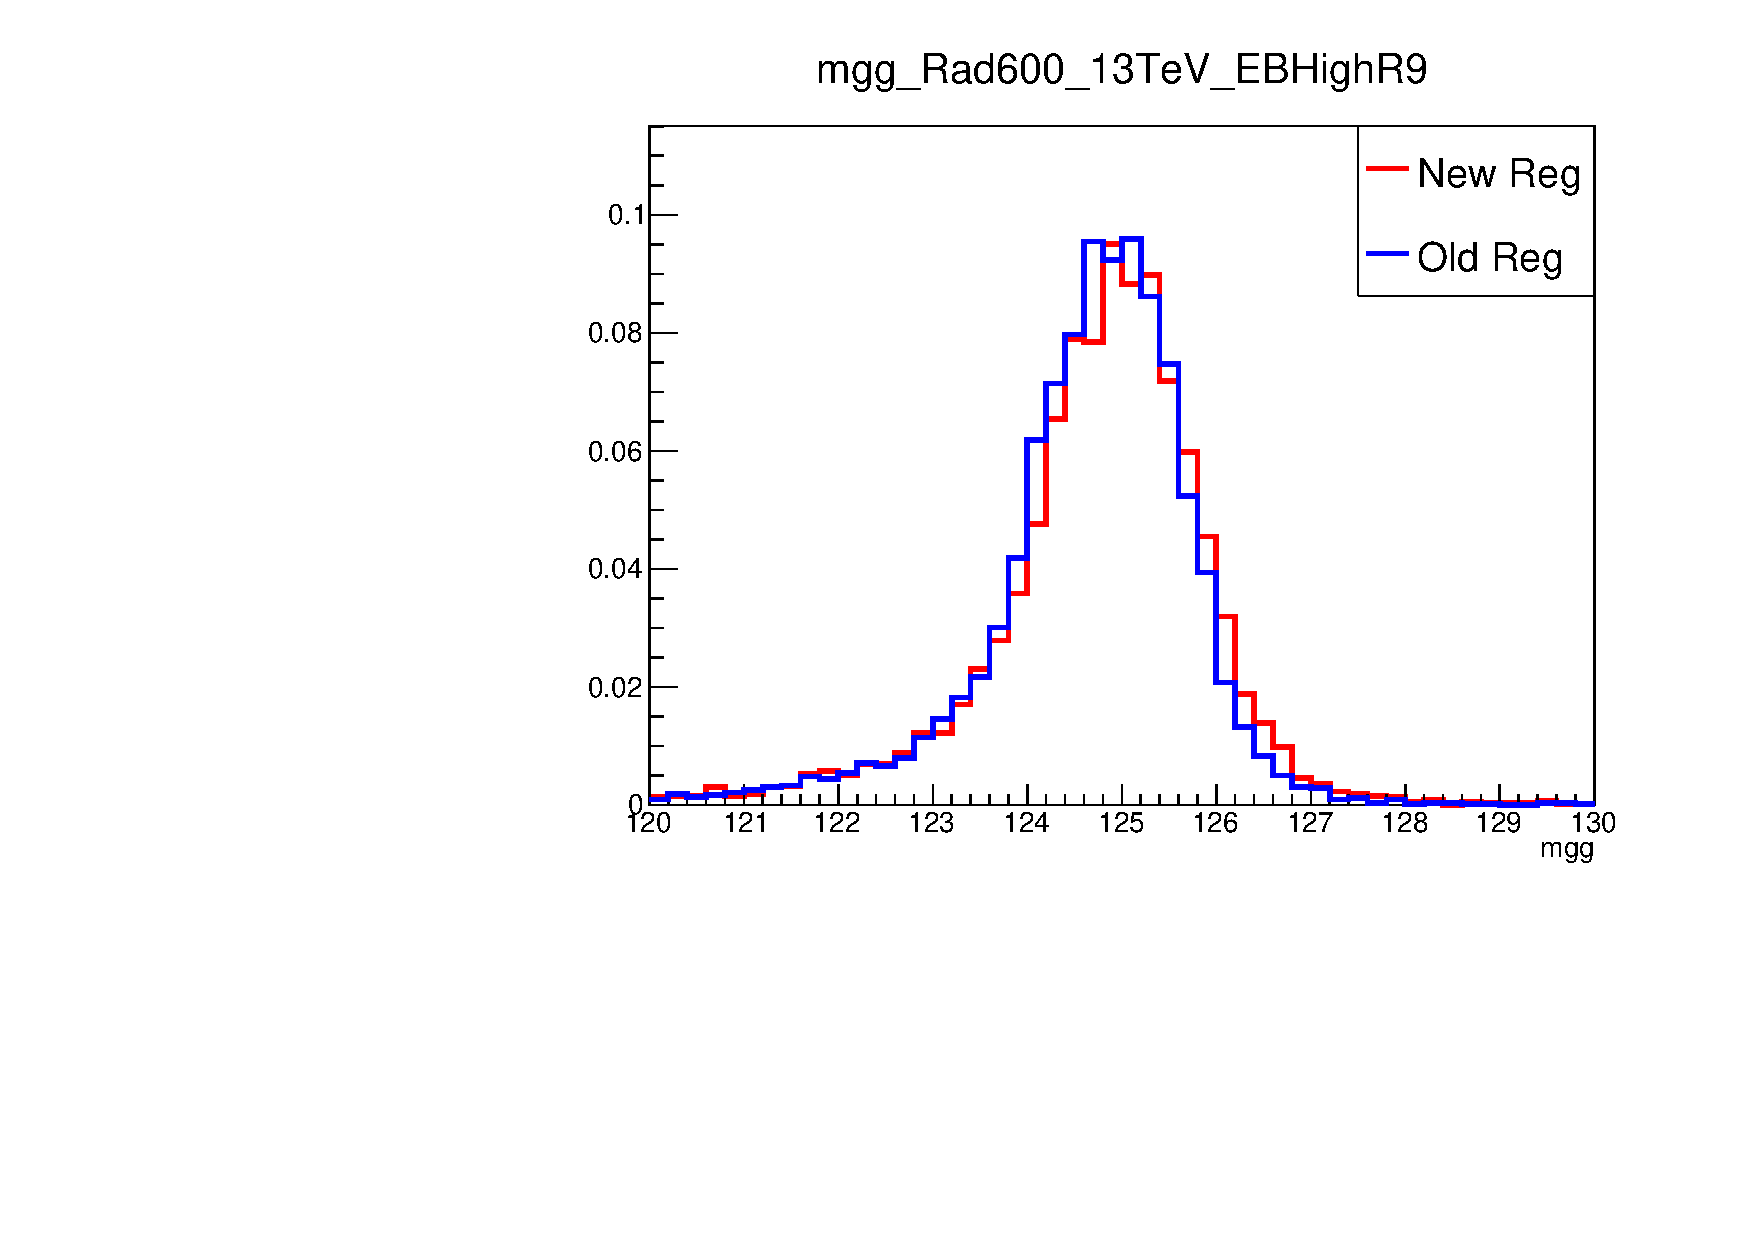
\includegraphics[trim={0 0 0 0.95cm},clip,width=0.3\textwidth]{figures/sec-photons/mgg_Rad600_13TeV_EBHighR9.pdf}\hfil
  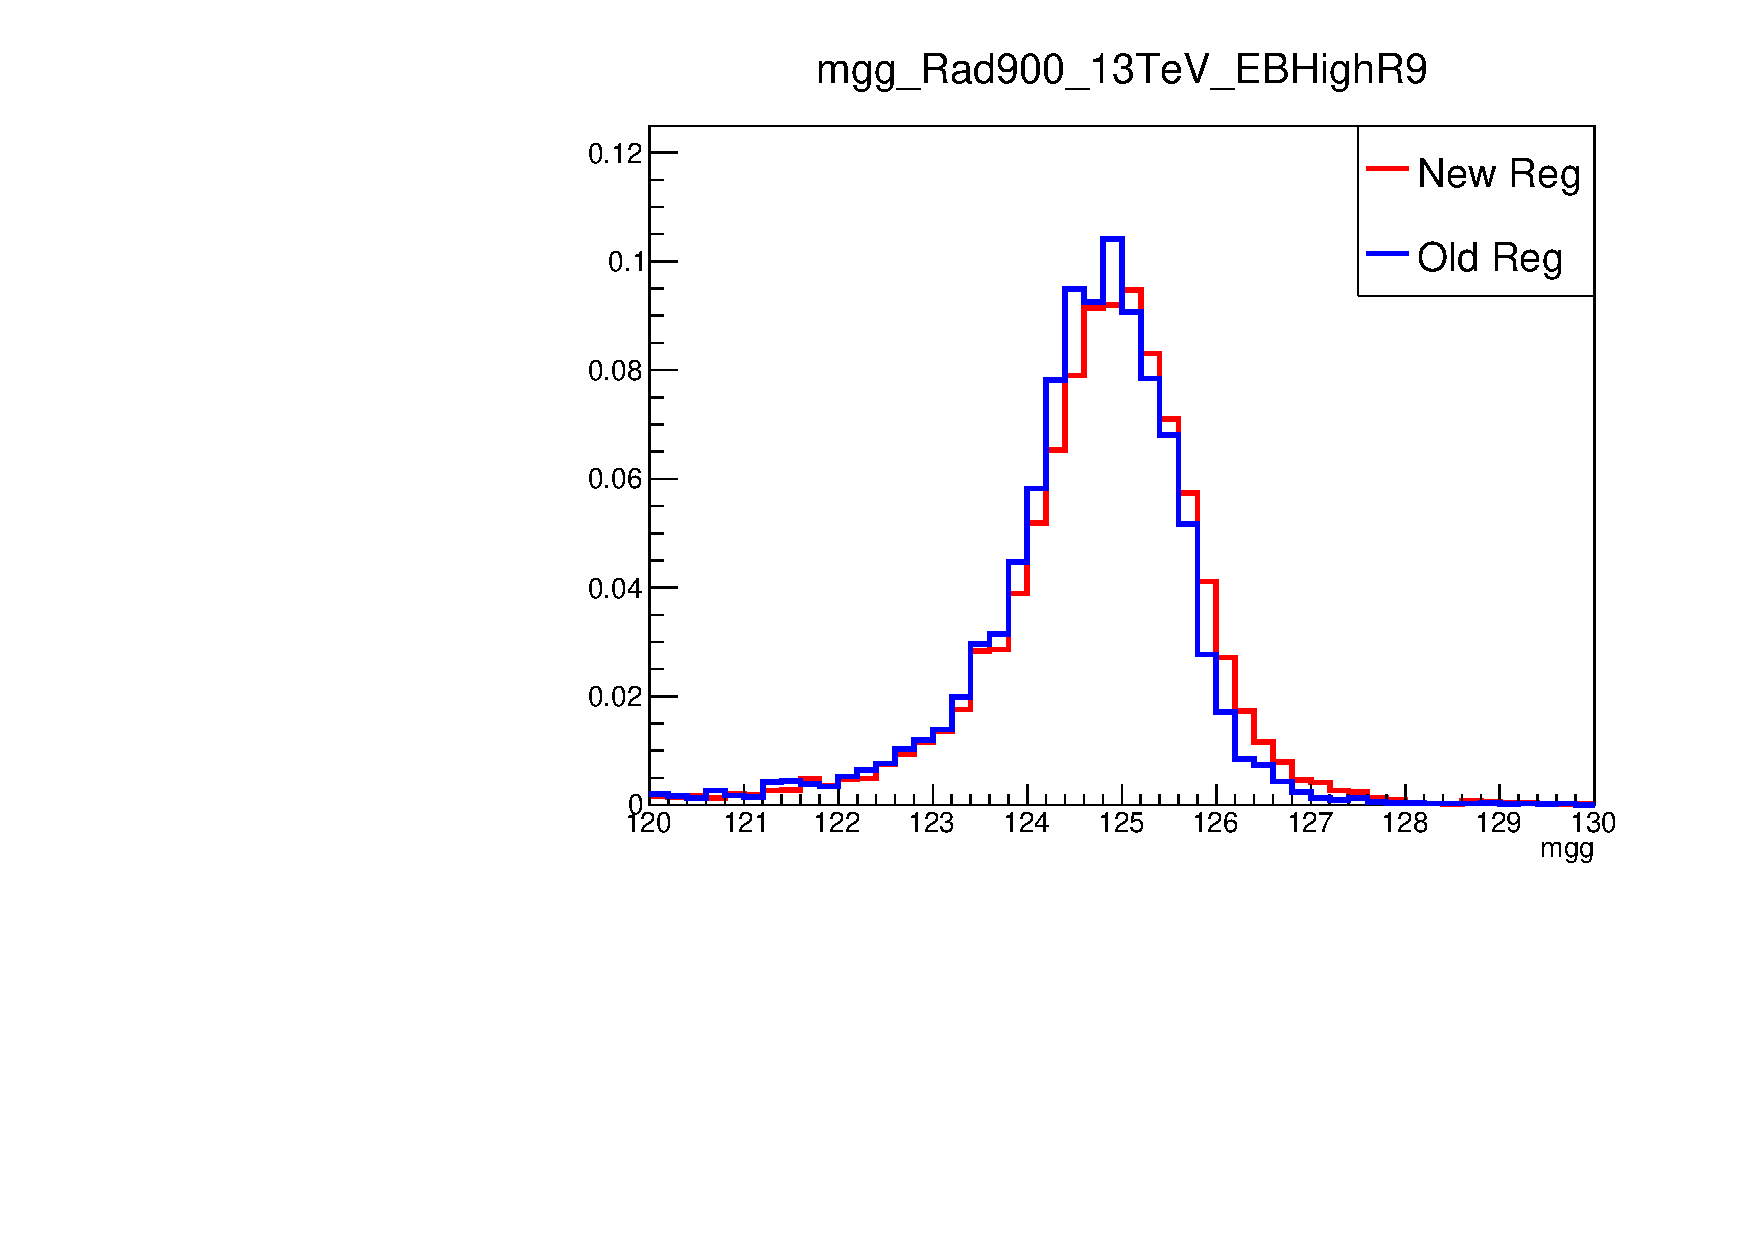
\includegraphics[trim={0 0 0 0.95cm},clip,width=0.3\textwidth]{figures/sec-photons/mgg_Rad900_13TeV_EBHighR9.pdf}\hfil
  \caption{$M(\gamma\gamma)$ reconstructed with different versions of the photon energy regression for resonance masses of 300, 600 and 900 GeV, from left to right. Distributions normalized to unity.}
  \label{fig:pho_reg}
\end{figure*}
